\section{Results}
\label{sec:results}

\subsection{RQ1: one compiled document}
\label{sec:res-single}
% See results/composition/distractor-curves/ for the untouched SQuAD evaluation.
As can be seen in Figure~\ref{fig:composition}, D2L falls below ICL even at
$K=1$, and adding distractors widens the gap. The trained readers recover only
part of the loss and do not prevent accuracy from declining as more documents
are added. We first examine the single-document gap.

% Question-mean point estimates; see results/composition/distractor-curves/.
% Qwen containment is plotted to avoid treating answer-format F1 gains as content gains.
\begin{figure}[t]
\centering
\begin{tikzpicture}
\begin{groupplot}[
 group style={group size=2 by 1,horizontal sep=0.75cm},
 scale only axis,width=0.34\columnwidth,height=2.7cm,
 xmode=log,log basis x=2,xtick={1,2,4,8,16},
 xticklabels={1,2,4,8,16},xmin=1,xmax=16,ymin=0,ymax=1,
 xlabel={Documents $K$},grid=major,
  tick label style={font=\scriptsize},label style={font=\scriptsize},
  title style={font=\scriptsize},
  legend style={font=\scriptsize,draw=none,legend columns=2}]
\nextgroupplot[title={Gemma-2-2B (F1)},ylabel={Token F1},legend to name=compositionlegend]
\addplot[black,mark=square*,thick] coordinates {(1,.872696)(2,.863)(4,.858)(8,.849)(16,.825)};
\addlegendentry{ICL}
\addplot[red!75!black,mark=*,thick] coordinates {(1,.755174)(2,.618)(4,.445)(8,.200)(16,.026)};
\addlegendentry{Native D2L}
\addplot[blue!75!black,mark=triangle*,thick] coordinates {(1,.755174)(2,.603575)(4,.421341)(8,.282533)(16,.228939)};
\addlegendentry{Normalized}
\addplot[teal!80!black,mark=diamond*,thick] coordinates {(1,.760839)(2,.624)(4,.465)(8,.268)(16,.117)};
\addlegendentry{Post-block reader}
\addplot[violet!80!black,mark=pentagon*,thick,dashed] coordinates {(1,.758)(2,.633)(4,.492)(8,.348)(16,.251)};
\addlegendentry{Write-site reader}
\addplot[orange!85!black,mark=x,thick,dashdotted] coordinates {(1,.750183)(2,.605258)(4,.417680)(8,.288555)(16,.184348)};
\addlegendentry{Gated reader}
\nextgroupplot[title={Qwen3-4B (containment)}]
\addplot[black,mark=square*,thick] coordinates {(1,.880213)(2,.876664)(4,.882875)(8,.891748)(16,.893523)};
\addplot[red!75!black,mark=*,thick] coordinates {(1,.683230)(2,.484472)(4,.321207)(8,.069210)(16,0)};
\addplot[blue!75!black,mark=triangle*,thick] coordinates {(1,.683230)(2,.433895)(4,.270630)(8,.197870)(16,.147294)};
\addplot[teal!80!black,mark=diamond*,thick] coordinates {(1,.633540)(2,.471162)(4,.342502)(8,.187223)(16,.072760)};
\addplot[orange!85!black,mark=x,thick,dashdotted] coordinates {(1,.619343)(2,.435670)(4,.271517)(8,.180124)(16,.104703)};
\end{groupplot}
\end{tikzpicture}
\par\smallskip\ref{compositionlegend}
\caption{Accuracy as the number of documents $K$ increases: token F1 for Gemma
and answer containment for Qwen. D2L falls below ICL already at $K=1$.
ICL stays relatively stable as distractors are added, while native D2L,
normalization, and the readers all degrade. All plotted readers are mixed-$K$.
Gemma includes all three readers; Qwen includes post-block and gated readers.
Gated readers use one seed, the other Gemma readers three.}
\label{fig:composition}
\end{figure}


\subsubsection{Retention and attribution (RQ1.1)}
% See results/single-document/answer-attribution/.
Using the answer-matching procedure described in Section~\ref{sec:diagnostics},
we compare incorrect responses with reference answers to other questions about
the same passage. Among teacher-correct questions each model misses, 46\% of
D2L's responses match another passage answer, compared with 10\% for the base
model. This describes passage-content attribution rather than a chance-corrected
binding error rate, since the base model has no document access.
The separate token-presence probe detects answer tokens in the
compiler latent even when generation fails, although it does not establish
whether those tokens survive conversion into LoRA factors.

\subsubsection{Readout and passage fitting (RQ1.2)}
% See results/single-document/reader-controls/ and passage-fitting/.
As shown in Table~\ref{tab:readout-summary}, the $K=1$-only post-block readers
improve over native D2L but remain below ICL. Using individual rank effects
gives only a small improvement over summed effects or compiler latents.
Changing reader width or layer sharing does not close the remaining gap.
Compiler fine-tuning and
question-conditioned writes reduce training losses without improving
accuracy on held-out questions.

\begin{table}[t]
\centering
\caption{Post-block readers improve on native D2L but remain below ICL.
The three readers are trained at $K=1$ only on gold answers.}
\label{tab:readout-summary}
\small
\begin{tabular}{@{}lr@{}}
\toprule
Readout & F1 \\
\midrule
ICL (baseline) & .882 \\
Native D2L & .755 \\
Reader: summed adapter effect & .781 \\
Reader: compiler latent & .785 \\
Reader: individual rank effects & .789 \\
\bottomrule
\end{tabular}
\end{table}


Fitting adapters separately to each passage also leaves overall accuracy close
to native D2L on the 160-passage set. Answers covered by the generated training
questions approach teacher accuracy, while uncovered answers become less
accurate. At the selected budget of ten forward-KL steps, increasing rank
from 8 to 64 does not reliably improve overall accuracy or prevent the
decline on uncovered answers.
Appendix~\ref{sec:single-tables} provides supporting results for answer
attribution, the latent probe, and passage fitting.

\subsubsection{The document read at the answer positions (RQ1.3)}
% The transplant and direct read mask were measured separately on the reused 402-question set.
As shown in Table~\ref{tab:causal}, replacing question-position states with
teacher states does not improve native D2L, whereas including answer-history
positions recovers part of the gap. Improving the question-position states
alone is therefore insufficient in this intervention.

The document-read masks in the same table show that both question and answer
positions contribute to ICL accuracy. Adding answer-position document reads
improves native D2L but does not reach the teacher, indicating that some of
the missing computation occurs during answer generation.

\begin{table}[t]
\centering
\caption{Effects of teacher-state transplants and document-attention masks
on answer accuracy. Gemma-2-2B, macro F1; each panel has its own measured baseline.}
\label{tab:causal}
\small
\begin{tabular}{@{}lr@{}}
\toprule
Intervention & F1 \\
\midrule
\multicolumn{2}{@{}l}{\emph{Hidden-state transplant}} \\
ICL (baseline) & .683 \\
Native D2L, self-transplant & .638 \\
Teacher states: question positions & .624 \\
Teacher states: question + answer history & .661 \\
\midrule
\multicolumn{2}{@{}l}{\emph{Direct document-read mask}} \\
ICL (baseline) & .688 \\
No positions read the document & .208 \\
Question positions only & .444 \\
Answer positions only & .427 \\
Native D2L & .633 \\
Native D2L + answer-position reads & .658 \\
\bottomrule
\end{tabular}
\end{table}

\subsection{RQ2: multi-document diagnostics}
\label{sec:res-composition}
\label{sec:res-gap}
\subsubsection{Composition and update size (RQ2.1)}
As can be seen in Figure~\ref{fig:composition}, adding distractors reduces
D2L accuracy substantially on both models, while ICL remains comparatively
stable. The normalization described in Section~\ref{sec:composition-diagnostics}
gives a modest improvement at larger bank sizes, while accuracy remains well
below ICL.

\subsubsection{Layer localization (RQ2.2)}
\label{sec:res-layers}
% See results/composition/layer-interventions/.
At $K=8$, applying the full bank in the initial layers gives similar measured
accuracy to withholding all document contributions there, with the source
alone applied in subsequent layers (Figure~\ref{fig:layers}(a)).
At layer 8 the two conditions reach .611 and .633 F1; at layer 13 they reach
.466 and .480. Interference accumulates across depth at this bank size,
whereas at $K=16$ retaining the full bank through layer 7 already reduces
F1 to .111, against .740 for the source alone.

Additionally, in Table~\ref{tab:prompt-interventions} we can see that delaying source application
until after prompt processing also reduces accuracy, despite using the known
source-only mask. Conversely, removing distractors only after prompt processing
does not recover the single-document result. The document contributions during
prompt processing therefore affect accuracy beyond the point at which the
adapters are changed.

\begin{table}[t]
\centering
\caption{Effects of delaying source application and distractor removal during
prompt processing. Gemma-2-2B, F1 at $K=8$. Cache replay updates cached
keys and values using source-induced residual corrections without fully
recomputing subsequent attention and MLP outputs.}
\label{tab:prompt-interventions}
\small
\begin{tabular}{@{}lr@{}}
\toprule
Condition & F1 \\
\midrule
ICL (baseline) & .870 \\
Native D2L, source alone & .740 \\
Native D2L, all documents & .198 \\
Uniform normalization & .301 \\
\midrule
\multicolumn{2}{@{}l}{\emph{Bank silent during prompt processing}} \\
Source at last prompt and response positions & .437 \\
Source applied with cache replay & .569 \\
\midrule
\multicolumn{2}{@{}l}{\emph{All documents active during prompt processing}} \\
Distractors removed at response positions & .313 \\
Also removed at last prompt position & .430 \\
\bottomrule
\end{tabular}
\end{table}

% Evidence in results/composition/layer-interventions/.
% Left: native-below-layer.json (native below L, K=8 and K=16; layers 0/8/18),
% cross-model-and-dataset-replication.json (native below L at layers 4/13/22; silent below L at layers 4/13),
% attenuation-schedules.json (silent below 8), and layer-six-ceiling.json (silent below 6); development set,
% 1,260 questions.
% Middle: per-question document-level membership AUC by layer, K=8: source-membership-probe.json
% (response positions, b_rows; also K=16) and clean-prefill-probe.json (clean prefill, prompt mean, b_rows).
% Right: cross-model-and-dataset-replication.json. Gate layer as a fraction of depth (26 Gemma, 36 Qwen
% layers); F1 as a fraction of the cell's native K=1 (0.740 SQuAD/Gemma, 0.385 DROP+ROPES/Gemma,
% 0.264 SQuAD/Qwen). Native below L: Gemma SQuAD 0/4/8/13/18/22; DROP+ROPES 0/8/18; Qwen 0/11/25.
% Silent below L: Gemma SQuAD 0/4/6/8/13; DROP+ROPES 6/8; Qwen 8/11.
\begin{figure}[t]
\centering
\begin{minipage}[t]{.49\columnwidth}
\vspace{0pt}
\centering
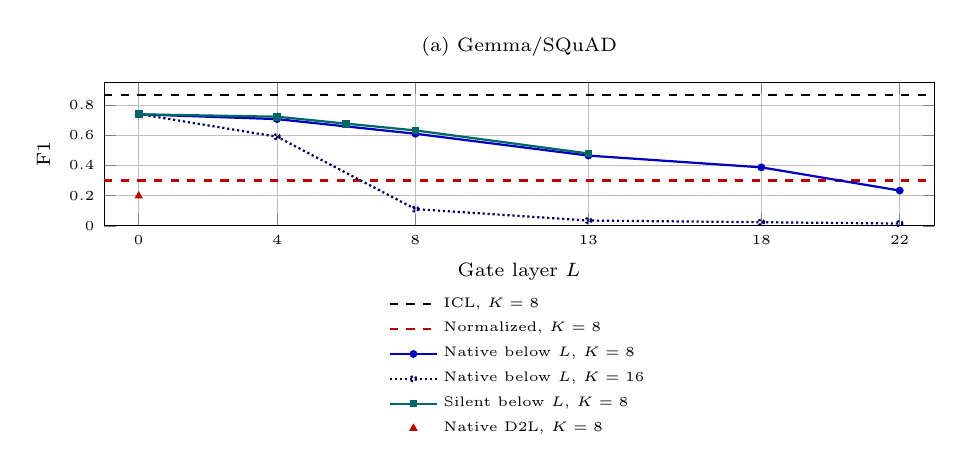
\begin{tikzpicture}
\begin{axis}[
 width=\linewidth,height=3.4cm,grid=major,
 tick label style={font=\tiny},label style={font=\scriptsize},
 title={(a) Gemma/SQuAD},title style={font=\scriptsize},
 mark size=1pt,
 xlabel={Gate layer $L$},
 ylabel={F1},xmin=-1,xmax=23,ymin=0,ymax=0.95,xtick={0,4,8,13,18,22},
  legend style={font=\tiny,draw=none,at={(0.5,-0.42)},anchor=north,
  legend columns=1,cells={anchor=west}}]
\addplot[black,dashed,thick] coordinates {(-1,.870)(23,.870)};
\addlegendentry{ICL, $K=8$}
\addplot[red!75!black,dashed,thick] coordinates {(-1,.301)(23,.301)};
\addlegendentry{Normalized, $K=8$}
\addplot[blue!75!black,mark=*,thick] coordinates {(0,.740)(4,.708)(8,.611)(13,.466)(18,.388)(22,.234)};
\addlegendentry{Native below $L$, $K=8$}
\addplot[blue!40!black,mark=o,thick,densely dotted] coordinates {(0,.742)(4,.591)(8,.111)(13,.035)(18,.024)(22,.015)};
\addlegendentry{Native below $L$, $K=16$}
\addplot[teal!80!black,mark=square*,thick] coordinates {(0,.740)(4,.724)(6,.678)(8,.633)(13,.480)};
\addlegendentry{Silent below $L$, $K=8$}
\addplot[red!75!black,mark=triangle*,thick,only marks] coordinates {(0,.198)};
\addlegendentry{Native D2L, $K=8$}
\end{axis}
\end{tikzpicture}
\end{minipage}\hfill
\begin{minipage}[t]{.49\columnwidth}
\vspace{0pt}
\centering
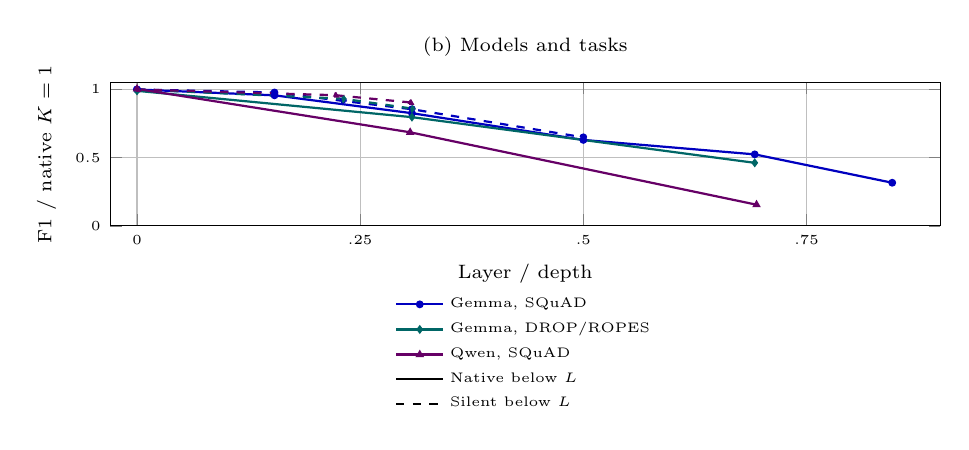
\begin{tikzpicture}
\begin{axis}[width=\linewidth,height=3.4cm,grid=major,
 tick label style={font=\tiny},label style={font=\scriptsize},
 title={(b) Models and tasks},title style={font=\scriptsize},
 xlabel={Layer / depth},ylabel={F1 / native $K=1$},
 xmin=-0.03,xmax=0.9,ymin=0,ymax=1.05,
 xtick={0,.25,.5,.75},xticklabels={0,.25,.5,.75},
 legend style={font=\tiny,draw=none,at={(0.5,-0.42)},anchor=north,
 legend columns=1,cells={anchor=west}},
 mark size=1pt]
\addplot[blue!75!black,mark=*,thick] coordinates {(0,1)(0.154,.957)(0.308,.826)(0.5,.630)(0.692,.524)(0.846,.316)};
\addlegendentry{Gemma, SQuAD}
\addplot[blue!75!black,mark=*,thick,dashed,forget plot] coordinates {(0,1)(0.154,.978)(0.231,.916)(0.308,.855)(0.5,.649)};
\addplot[teal!80!black,mark=diamond*,thick] coordinates {(0,.990)(0.308,.797)(0.692,.462)};
\addlegendentry{Gemma, DROP/ROPES}
\addplot[teal!80!black,mark=diamond*,thick,dashed,forget plot] coordinates {(0,1)(0.231,.932)(0.308,.860)};
\addplot[violet!80!black,mark=triangle*,thick] coordinates {(0,1.004)(0.306,.686)(0.694,.155)};
\addlegendentry{Qwen, SQuAD}
\addplot[violet!80!black,mark=triangle*,thick,dashed,forget plot] coordinates {(0,1)(0.222,.958)(0.306,.905)};
\addlegendimage{black,thick}
\addlegendentry{Native below $L$}
\addlegendimage{black,thick,dashed}
\addlegendentry{Silent below $L$}
\end{axis}
\end{tikzpicture}
\end{minipage}
\caption{Layer sensitivity to distractors. (a) Absolute F1 on Gemma/SQuAD.
(b) Across models and tasks at $K=8$, normalized by model depth and native
$K=1$ accuracy. Distractors are removed from layer $L$ onward.}
\label{fig:layers}
\label{fig:layer-generality}
\end{figure}

\begin{figure}[t]
\centering
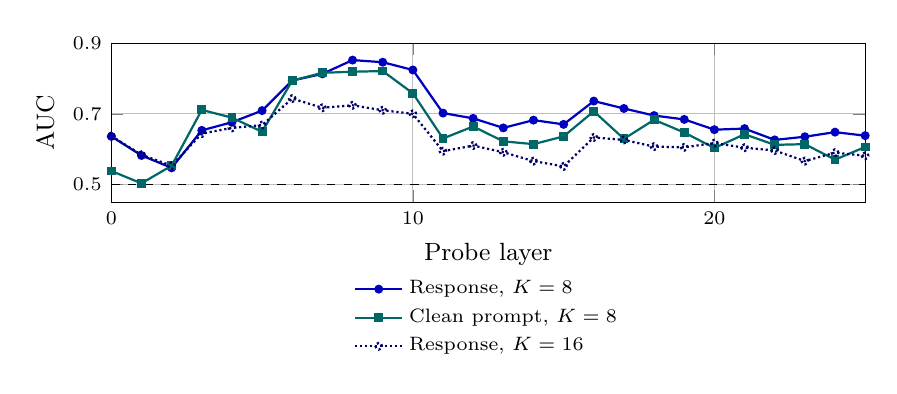
\begin{tikzpicture}
\begin{axis}[width=.92\columnwidth,height=3.6cm,grid=major,
 tick label style={font=\scriptsize},label style={font=\small},
 xlabel={Probe layer},ylabel={AUC},
 xmin=0,xmax=25,ymin=.45,ymax=.9,
 xtick={0,10,20},ytick={.5,.7,.9},
 legend style={font=\scriptsize,draw=none,at={(0.5,-0.42)},anchor=north,
 legend columns=1,cells={anchor=west}}]
\addplot[black,dashed,thin,forget plot] coordinates {(0,.5)(25,.5)};
\addplot[blue!75!black,mark=*,mark size=1.2pt,thick] coordinates {
(0,.636)(1,.582)(2,.547)(3,.653)(4,.676)(5,.709)(6,.794)(7,.813)(8,.852)(9,.846)(10,.824)
(11,.702)(12,.687)(13,.660)(14,.682)(15,.670)(16,.736)(17,.715)(18,.695)(19,.684)(20,.655)
(21,.658)(22,.626)(23,.635)(24,.648)(25,.638)};
\addlegendentry{Response, $K=8$}
\addplot[teal!80!black,mark=square*,mark size=1.2pt,thick] coordinates {
(0,.538)(1,.503)(2,.553)(3,.711)(4,.689)(5,.649)(6,.794)(7,.816)(8,.819)(9,.821)(10,.758)
(11,.630)(12,.664)(13,.622)(14,.614)(15,.636)(16,.707)(17,.629)(18,.683)(19,.647)(20,.603)
(21,.642)(22,.612)(23,.614)(24,.570)(25,.606)};
\addlegendentry{Clean prompt, $K=8$}
\addplot[blue!40!black,mark=o,mark size=1.2pt,thick,densely dotted] coordinates {
(0,.637)(1,.584)(2,.553)(3,.644)(4,.660)(5,.668)(6,.743)(7,.717)(8,.724)(9,.710)(10,.700)
(11,.594)(12,.610)(13,.591)(14,.566)(15,.551)(16,.633)(17,.626)(18,.607)(19,.605)(20,.617)
(21,.604)(22,.596)(23,.566)(24,.590)(25,.581)};
\addlegendentry{Response, $K=16$}
\end{axis}
\end{tikzpicture}
\caption{Source-membership predictability by layer. Probe AUC on Gemma;
the dashed line marks chance.}
\label{fig:layer-probes}
\end{figure}


\label{sec:res-generality}
Figure~\ref{fig:layer-generality}(b) shows a similar pattern across models and
datasets: removing distractors earlier preserves more accuracy, while
withholding early source contributions also reduces accuracy.
However, the preregistered criterion that the loss at one-third depth reach
at least half the loss at two-thirds depth is not met: the observed fraction
is .36--.37 across all three model/task evaluations.

\subsubsection{Membership probes and gates (RQ2.3)}
\label{sec:res-probes}
Using the membership probes described in Section~\ref{sec:composition-diagnostics},
we measure how well each layer's hidden state and rank keys distinguish the
source from distractors. As shown in Figure~\ref{fig:layer-probes}, source membership is most readily
predicted around layers 6--10 on Gemma. Figure~\ref{fig:layers} shows that
document contributions in the preceding layers already affect answer accuracy,
so the strongest membership predictions become available after interference
has begun. The clean-prompt probe shows that source membership is also
detectable without first applying the document bank.

\subsubsection{Trained readers (RQ2.3)}
\label{sec:res-readers}
As shown in Figure~\ref{fig:composition}, none of the readers managed to learn
to reliably separate query-dependent facts from distractors.

On Qwen, the gated reader improves token F1 but reduces answer containment
at $K=1$. Its containment is close to normalization at $K=2,4,8$ and lower
at $K=16$, so the F1 gains do not establish better fact retention.

The localization results do not explain the reader failures by timing alone.
At $K=8$, a source-only oracle applied from layer 8 retains .611 F1 on the
development set, despite interference in the preceding layers. There is
therefore substantial scope for correction at intermediate depth; the tested
readers do not establish that this scope can be realized through their
architectures and training objectives.

\subsection{RQ3: D2L on MidBrain}
\label{sec:res-delivers}

\subsubsection{MidBrain on PersonaMem-v2}
% See results/deployment/personamem/; question-weighted, persona-cluster bootstrap.
\begin{table}[t]
\centering
\caption{MidBrain on PersonaMem-v2. Qwen3-4B accuracy and median memory
tokens per request. Adapter conditions retain the same retrieved episodes as text.}
\label{tab:user-memory-summary}
\small\setlength{\tabcolsep}{3pt}
\begin{tabular}{@{}lrr@{}}
\toprule
Memory representation & Accuracy & Tokens \\
\midrule
Full history as text (baseline) & .364 & 31{,}847 \\
\midrule
Episodic (text) & .376 & 8{,}736 \\
Consolidated (text) & .353 & 1{,}451 \\
Episodic + consolidated (text) & .390 & 10{,}159 \\
Episodic + consolidated (LoRA) & .391 & 8{,}736 \\
Episodic + consolidated (LoRA sum) & .274 & 8{,}736 \\
Episodic + consolidated (LoRA norm.) & .387 & 8{,}736 \\
\bottomrule
\end{tabular}
\end{table}

As shown in Table~\ref{tab:user-memory-summary}, compiling consolidated memory
jointly preserves similar measured accuracy to supplying it as text.
Summing separately compiled adapters substantially reduces accuracy even
with episodic text available. Normalization recovers most of this loss,
bringing accuracy close to joint compilation and text memory.
It should be noted that absolute scores are not directly comparable with the original PersonaMem-v2
evaluation because our protocol omits generated reasoning.

\subsubsection{Serving cost}
% See results/deployment/serving-cost/. MACs, not FLOPs.
% Analytical MACs: tab:cost-length. Measured throughput: tab:throughput.
\begin{figure}[t]
\centering
\begin{tikzpicture}
\begin{groupplot}[group style={group size=2 by 1,horizontal sep=1.2cm},
 scale only axis,width=.31\columnwidth,height=2.6cm,grid=major,
 tick label style={font=\scriptsize},label style={font=\scriptsize},
 title style={font=\scriptsize},
 legend style={font=\scriptsize,draw=none,at={(.5,-.28)},anchor=north,legend columns=1}]
\nextgroupplot[title={(a) Analytical compute},
 xlabel={Memory tokens},ylabel={GMAC/request (log)},
 xmode=log,log basis x=2,ymode=log,
 xtick={150,1024,4096},xticklabels={150,1024,4096},
 ymin=100,ymax=20000]
\addplot[black,dashed,mark=square*,thick] coordinates {(150,583)(512,1544.8)(1024,2929.1)(2048,5781.3)(4096,11820.7)};
\addlegendentry{ICL: full prefill}
\addplot[teal!80!black,mark=diamond*,thick] coordinates {(150,188.8)(512,188.8)(1024,188.8)(2048,188.8)(4096,188.8)};
\addlegendentry{Native D2L}
\nextgroupplot[title={(b) Batched serving throughput},
 xlabel={Batch size},ylabel={Aggregate tokens/s},
 xtick={1,8,16},xmin=0,xmax=17,ymin=0,ymax=350]
\addplot[teal!80!black,dashed,mark=diamond*,thick] coordinates {(1,24.3)(8,165.3)(16,290.9)};
\addlegendentry{Gemma ICL}
\addplot[teal!80!black,mark=diamond*,thick] coordinates {(1,20.1)(8,157.8)(16,315.8)};
\addlegendentry{Gemma D2L}
\addplot[blue!75!black,dashed,mark=triangle*,thick] coordinates {(1,21.5)(8,122.0)(16,162.5)};
\addlegendentry{Qwen ICL}
\addplot[blue!75!black,mark=triangle*,thick] coordinates {(1,17.1)(8,134.9)(16,269.4)};
\addlegendentry{Qwen D2L}
\end{groupplot}
\end{tikzpicture}
\caption{Recurring compute and serving throughput. (a) Gemma, one document,
40 question tokens and 32 output tokens. (b) One A100, four documents per user
and 64 output tokens per user. Each batch contains one request per user,
with distinct user-specific memory. Throughput includes prefill and decoding;
ICL performs full prefill per request. Compilation is excluded.}
\label{fig:serving-tradeoff}
\end{figure}


As shown in Figure~\ref{fig:serving-tradeoff}(a), D2L's recurring compute
advantage grows with document length: ICL processes more document tokens,
whereas the compiled adapter has fixed size. These estimates cover
request-time prefill and decoding, excluding compilation.

As shown in Figure~\ref{fig:serving-tradeoff}(b), increasing batch size from
1 to 16 raises D2L's throughput relative to ICL from $0.83\times$ to
$1.09\times$ on Gemma and from $0.80\times$ to $1.66\times$ on Qwen.
We hypothesize that batching amortizes model-weight reads and execution
overhead, making the cost of ICL's longer contexts more prominent.
At small batch sizes, the additional LoRA operations may instead cost more
time than the document computation they replace, particularly when execution
is limited by memory access or kernel-launch overhead rather than arithmetic.
